\documentclass{article}
\usepackage[utf8]{inputenc}
\usepackage{amsmath} 
\usepackage{enumitem}
\usepackage{graphicx}
\usepackage{mathtools}
\newcommand{\ddt}[1]{\frac{\partial #1}{\partial t}}
\newcommand{\dddt}[1]{\frac{\partial^2 #1}{\partial t^2}}
\newcommand{\ddx}[1]{\frac{\partial #1}{\partial x}}
\newcommand{\dddx}[1]{\frac{\partial^2 #1}{\partial x^2}}
\newcommand{\bracket}[1]{\left[ #1 \right]}
\newcommand{\paren}[1]{\left( #1 \right)}
\newcommand{\braket}[1]{\left\langle #1 \right\rangle}

\title{Chapter 1 Problems}
\author{William Arnold}
\date\today

\begin{document}
\maketitle 

\section*{Problem 1.1}
For the distribution of ages in the example in Section 1.3.1
\begin{align*}
  N(14) &= 1 \\
  N(15) &= 1 \\
  N(16) &= 3 \\
  N(22) &= 2 \\
  N(24) &= 2 \\
  N(25) &= 5
\end{align*}

\begin{enumerate}[label=(\alph*)]
  \item Compute $\braket{j^2}$ and $\braket{j}^2$
    Total number of kids is $1 + 1 + 3 + 2 + 2 + 5 = 14$. 
    \begin{align*}
      \braket{j^2} &= \frac{1}{14}(14^2 + 15^2) + \frac{2}{14}(22^2 + 24^2) + \frac{3}{14}16^2 + + \frac{5}{14}25^2 \\
                   &= \frac{3217}{7} \approx 459.57  \\
      \braket{j} &= \frac{1}{14}(14 + 15) + \frac{2}{14}(22 + 24) + \frac{3}{14}16 + + \frac{5}{14}25 \\
                   &= 21 \\
      \braket{j}^2 &= 441
    \end{align*}
  \item Determine $\Delta j$ for each $j$ and use Equation 1.11 to compute the standard deviation
    \begin{align*}
      \sigma^2 &= \braket{(\Delta j)^2} = \frac{1}{14}((-7)^2 + (-6)^2) + \frac{2}{14}(1^2 + 3^2) + \frac{3}{14}(-5)^2 + + \frac{5}{14}4^2 \\
               &= \frac{130}{7}
    \end{align*}

  \item Check using part a and part b 
    \begin{align*}
      \sigma^2 &= \braket{j^2} - \braket{j}^2 = \frac{130}{7} \\
               &= \braket{(\Delta j)^2} 
    \end{align*}
\end{enumerate}

\newcommand{\intinf}{\int_{-\infty}^\infty}
\newcommand{\intzinf}{\int_{0}^\infty}

\section{Problem 1.3}
  Consider the Gaussian Distribution
  \[
    \rho(x) = Ae^{-\lambda (x - a)^2}
  \]
  where $A, a$ and $\lambda$ are positive real constants (necessary integrals are in the back of the book)
  \begin{enumerate}[label=(\alph*)]
    \item Use equation 1.16 to determine $A$
      We have that $\intinf \rho(x) = 1$ so we have 
        \begin{align*}
          \intinf Ae^{-\lambda (x - a)^2} dx &= 2A\intzinf e^{-\lambda x^2} dx \\
                                                             &= 2A\sqrt{\pi}\frac1{2\sqrt{\lambda}} \\
                                                             &= A \sqrt{\frac\pi{\lambda}} = 1
        \end{align*}
        Thus solving for $A$ we get
        \[ A = \sqrt{\frac\lambda{\pi}} \]

    \item Find $\braket{x}, \braket{x^2}$, and $\sigma$
     
      Let $u = x-a$. Then $\frac{du}{dx} = 1, du = dx$, and
      \begin{align*}
        \braket{x} &= \intinf Axe^{-\lambda (x - a)^2}dx \\
                   &= \intinf A(u + a)e^{-\lambda u^2}du \\
                   &= \intinf Aue^{-\lambda u^2}du + \intinf Aae^{-\lambda u^2}du \\
      \end{align*}
      Since the first integral in the sum is integrating an odd function ($ue^{\lambda u^2} = -( (-u)e^{\lambda (-u)^2})$), that integral is zero. This leaves
      \begin{align*}
        \braket{x} &= \intinf Aae^{-\lambda u^2}du \\
                   &= a \intinf Ae^{-\lambda u^2}du \\
                   &= a
      \end{align*}
      
      Using the formula in the back of the book, we have that
      \begin{align*}
        \braket{x^2} &= \intinf x^2 Ae^{-\lambda (x - a)^2} dx \\
                     &= \intinf (u + a)^2 Ae^{-\lambda u^2} du \\
                     &= \intinf u^2 A e^{-\lambda u^2}du + \intinf 2auAe^{-\lambda u^2}du + \intinf a^2Ae^{-\lambda u^2}du \\
                     &= 4A\sqrt{\pi}(\frac{1}{2\sqrt{\lambda}})^3  + a^2 \\
                     &= \frac{1}{2} \frac{\sqrt\lambda}{\sqrt\pi} \sqrt{\pi} \frac{1}{\sqrt{\lambda}^3} + a^2 \\
                     &= \frac{1}{2 \lambda} + a^2
      \end{align*}
      And lastly, 
      \begin{align*}
        \sigma^2 = \braket{x^2} - \braket{x}^2 = \frac{1}{2\lambda} + a^2 - a^2 = \frac{1}{2\lambda}
      \end{align*}
  \end{enumerate}


\section{Problem 1.5}
  Consider the Gaussian wave function
  \[ \Psi(x, t) = Ae^{-\lambda |x|}e^{-i\omega t} \]
  Where $A, \omega,$ and $\lambda$ are real coefficients.

  \begin{enumerate}[label=(\alph*)]
    \item Normalize $\Psi$

      Firstly, $|\Psi| = |Ae^{-\lambda|x|}|$ since $|e^{i\omega t}| = |cos(\omega t) + i sin(\omega t)| = 1$.
      Thus $|\Psi|^2 = A^2 e^{-2\lambda|x|}$ so
      \begin{align*}
        \intinf |\Psi|^2 dx &= \intinf A^2 e^{-2\lambda |x|} dx \\
                            &= 2A^2 \intzinf e^{-2 \lambda x} dx \\
                            &= 2A^2 \frac{1}{-2\lambda} \intzinf e^{-2 \lambda x} (-2 \lambda) dx \\
                            &= 2A^2 \frac{1}{-2\lambda} \int_{0}^{-\infty} e^{u}du \\
                            &= \frac{2A^2}{-2 \lambda} [e^u]_0^{-\infty} \\
                            &= \frac{A^2}{-\lambda} (0 - 1) = \frac{A^2}{\lambda} = 1
      \end{align*}
      Thus, we have that $A = \sqrt{\lambda}$ and $\Psi$ is normalized.

    \item Determine $\braket{x}$ and $\braket{x^2}$
      \begin{align*}
        \braket{x} = \intinf x|\Psi|^2 dx &= \intinf \frac{x}{\lambda} e^{-2\lambda|x|}dx \\
                             &= \frac1\lambda \intinf x e^{-2 \lambda |x|} dx \\
                             &= 0 
      \end{align*}
      The last step follows from integrating an odd function symmetrically around 0. Now to find $\braket{x}^2$:
      \begin{align*}
        \braket{x}^2 = \intinf x^2|\Psi|^2 dx &= \frac1\lambda \intinf x^2 e^{-2\lambda|x|}dx \\
                                              &= \frac2\lambda \intzinf x^2 e^{-2\lambda x} dx \\
                                              &= \frac2\lambda 2 (\frac1{2\lambda})^3 \\
                                              &= \frac1{2\lambda ^4} 
      \end{align*}

    \item Find the standard deviation of $x$. 
      Sketch the graph of $|\Psi|^2$, as a function of $x$, and mark the points $(\braket{x} + \sigma)$ and $(\braket{x} - \sigma)$, to illustrate the sense in which $\sigma$ represents the "spread" in x.
      What is the probability that the particle would be found outside this range?

      Firstly, $\sigma^2 = \frac1{2\lambda^4}$ so $\sigma = \frac1{\sqrt{2\lambda}}$. Looking at a graph of $|\Psi|^2$ for $\lambda = 1$ marked at $x=\sqrt{\frac12}, -\sqrt{\frac12}$:

      \centerline{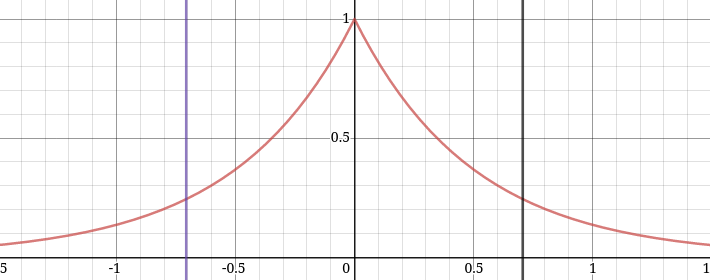
\includegraphics[width=6in]{1-5c.png}}

      The probability $x$ is greater than $\sqrt{\frac12}$ is
      \[\int_{0.5}^\infty e^{-2x}dx = \left[ -\frac12e^{-2x} \right]_{(1/\sqrt{2})}^{\infty} = \frac1{2e^{\sqrt2}} \approx 0.12156 \] 
      And the same value is taken for the probability than $x$ is less than $\sqrt{\frac12}$ by symmetry.
      Thus the probability that $x \notin [\braket{x} - \sigma, \braket{x} + \sigma]$ is $\frac1e^{\sqrt{2}} \approx 0.24312$.
  \end{enumerate}


\section{Problem 1.7}
Calculate $\frac{d\braket{p}}{dt}$. This should equal $\braket{-\frac{\partial V}{\partial x}}$.
\begin{align*}
  \frac{d\braket{p}}{dt} &= -i\hbar \intinf \paren{\ddt{\Psi^*} \ddx{\Psi} + \Psi^* \frac{\partial^2 \Psi}{\partial t \partial x}}dx
\end{align*}
First simplifying the second term in the integral we find
\begin{align*}
  \intinf \Psi^* \frac{\partial^2 \Psi}{\partial t \partial x} &= \bracket{\Psi^* \ddt\Psi}^{\infty}_{-\infty} - \intinf \ddx{\Psi^*} \ddt{\Psi} dx \\
                                                               &= \intinf \ddx{\Psi^*} \ddt{\Psi} dx
\end{align*}
Thus
\begin{align*}
  \frac{d\braket{p}}{dt} &= \intinf \bracket{\paren{i\hbar \ddt{\Psi}}^* \ddx{\Psi} + \ddx{\Psi^*}\paren{i\hbar\ddt{\Psi}}}dx \\
                         &= \intinf \bracket{\paren{-\frac{\hbar^2}{2m} \dddx{\Psi} + V \Psi}^*\ddx{\Psi} + \ddx{\Psi^*} \paren{-\frac{\hbar^2}{2m} \dddx{\Psi} + V \Psi}}dx \\
                         &= \intinf \bracket{-\frac{\hbar^2}{2m} \paren{\dddx{\Psi^*} \ddx\Psi + \ddx{\Psi^*} \dddx\Psi} + V \Psi^* \ddx\Psi + \ddx{\Psi^*} V \Psi}dx \\
                         &= \intinf \bracket{-\frac{\hbar^2}{2m} \ddx{} \paren{\ddx{\Psi^*} \ddx{\Psi}} + V \ddx{|\Psi|^2}}dx \text{\; (using the product rule) } \\
                         &= \frac{-\hbar^2}{2m}\bracket{\ddx{\Psi^*}\ddx\Psi}^\infty_{-\infty} + \intinf V \ddx{|\Psi|^2}dx \\
                         &= \intinf V \ddx{|\Psi|^2}dx \text{\; (since $\Psi$ and its derivatives vanish at infinity)}\\
                         &= \bracket{V|\Psi|^2}^\infty_{-\infty} - \intinf \ddx{V}|\Psi|^2 dx \text{\; (using integration by parts)} \\
                         &= \braket{-\ddx{V}}
\end{align*}

\end{document}

